The pad resonances discussed in Chapter~2 provide the main motivation for modifying the antenna feeding structure with resistive elements. To evaluate this concept systematically, a well-established H-Dipole
antenna design proposed in \cite{nandiErAsInAlGaAsPhotoconductors2021} is used as the reference geometry. Building upon this baseline, NiCr segments are selectively introduced into the antenna feeds in order to damp low-frequency surface currents. In the following, the design of the reference H-Dipole, the NiCr modifications and the simulation parameters are described. Only H-Dipoles are explicitly simulated. The results offer insight into the expected behavior of I-shaped Dipole antennas due to their structural similarities. 

\subsection{Design of Reference Antenna}

The reference antenna design consists of a metallic H-Dipole deposited on an active photoconductive layer of approximately \num{1.5} \si{\micro\meter} thickness. Beneath this active layer lies a semi-insulating Fe:InP substrate with a thickness of roughly \num{500} \si{\micro\meter}. To improve THz signal out-coupling, a hyper-hemispherical silicon lens with a radius of \num{6.1} \si{\milli\meter} is attached to the back side of the substrate. Simulating the entire geometry including the silicon lens is computationally infeasible. Therefore, a simplification technique described in \cite{llombartTHzTimeDomainSensing2012,garufoNortonEquivalentCircuit2018} is applied: the antenna is positioned at the air–substrate interface, and the simulation domain is truncated using appropriate boundary conditions. The "open add space" boundary condition is applied in the direction normal to the substrate, while "open" boundary conditions are used elsewhere to absorb outgoing electromagnetic waves and approximate an infinite domain.

The substrate thickness is set to be at least one wavelength across all relevant frequencies, ensuring realistic far-field behavior. The antenna is excited via a discrete port placed directly on the substrate. To maintain accuracy, the port dimensions are chosen to be at least five times smaller than the effective wavelength, which holds true for all frequencies up to \num{1} \si{\tera\hertz} considered here. The dimensions used for the H-Dipole antenna can be taken from Figure \ref{fig:sim_dimensions}. The deposited metal in the reference antenna is modeled as a perfectly electrically conducting (PEC) material. This approximation is valid, as gold is commonly used for THz antenna fabrication. Gold can be treated as a perfect conductor in the simulation frequency range.

\begin{figure}[!]
    \centering
        \begin{subfigure}[c]{0.45\textwidth}
        \centering
        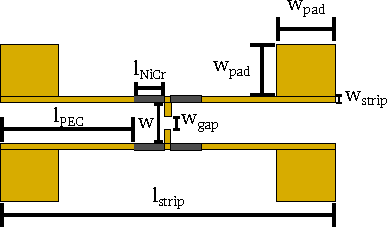
\includegraphics[width=\linewidth]{figures/sim_NICR_abmessungen.pdf}
        \label{fig:NICR}
    \end{subfigure}
    \hspace{0.1em}
    \begin{subtable}[c]{0.45\textwidth}
        \centering
        \begin{tabular}{ll}
        \toprule
        Variable & Length [$\mu m$]\\
        \midrule
        l\textsubscript{strip} & 1900 \\
        w\textsubscript{gap} & 5 \\
        w & 15 \\
        w\textsubscript{strip} & 5 \\
        w\textsubscript{pad} & 200 \\
        l\textsubscript{NiCr} & var. \\
        l\textsubscript{PEC} & var. \\
        \bottomrule
        \end{tabular}
        \label{tab:table1}
    \end{subtable}
    \caption{Important antenna dimensions used for simulation of H-Dipoles. l\textsubscript{NiCr} is set to zero when simulating the reference H-Dipole antenna.}
    \label{fig:sim_dimensions}
\end{figure}

\subsection{Design of NiCr-Modified Antennas}

To investigate the impact of incorporating resistive materials into the antenna feed, the reference H-Dipole topology is systematically modified by introducing NiCr strips into the feeding structure. For a meaningful comparison with the reference design, all other structural and simulation parameters are kept identical to those described previously.
NiCr is defined as an ohmic sheet material with a sheet resistance of \num{22} \si{\ohm/sq} in CST.

In the modified design, segments of the original perfectly electrically conducting (PEC) feeding lines are selectively replaced by NiCr. The integration of NiCr begins at the antenna’s electrodes, such that increasing the NiCr length moves the resistive section closer to the antenna’s contact pads. In CST, this is done by defining a length $l_{NiCr}$ that can be modified at will. Additionally, the length of the complete feeding strip $l_{strip}$ consists of the portion of the strip made up of PEC $l_{PEC}$ and the portion of the strip made up of the NiCr sheet $l_{NiCr}$. The values of $l_{PEC}$ and $l_{NiCr}$ always need to add up to $l_{strip}$, which is \num{1900} \si{\micro\meter} in this case. For efficient simulations where many possible values of $l_{NiCr}$ are to be evaluated, $l_{PEC}$ is defined as $l_{PEC} = l_{strip}/2 - l_{NiCr}$. This definition ensures that increasing the length of $l_{NiCr}$ automatically decreases the length of $l_{PEC}$, allowing the overall geometry of the feeding strip to remain constant across all configurations.


The resistance of the NiCr section is directly proportional to its length, as given by the relation: $R_{NiCr} \propto l_{NiCr}$. Thus, multiple configurations with varying strip lengths $l_{NiCr}$ are simulated in order to evaluate their impact on antenna performance and determine suitable parameters for future fabrication.

\subsection{Simulation Parameters}

Simulations are carried out using CST Studio Suite’s time-domain solver, which employs the finite integration technique (FIT) to solve Maxwell’s equations. A hexahedral mesh is used, and the simulation accuracy is set to \num{-30} \si{\decibel}. Field monitors are implemented at two distinct frequencies: \num{100} \si{\giga\hertz} and \num{1} \si{\tera\hertz}. At these frequencies, the electromagnetic field distribution is recorded. Monitors for the electric field, magnetic field, and surface current are used to analyze the antenna's radiation characteristics and internal behavior.
